\section{Results: Europe and United States}
\label{res}

%There is moderate interest in grid integration strategies in the United States, and low interest in the same in Europe. From the point of view of SCs, strategies such as cutting jobs or load migration have little interest. \\

%From our questionnaire, we concluded that neither European nor the United States sites are engaged with peak shedding, peak shifting or dynamic pricing programs at present. More sites in the United States have communicated with their ESPs regarding these programs. While both European and United States SCs are interested in dynamic pricing, there is mixed interest in peak shedding and peak shifting. The European sites are more interested in peak shedding than peak shifting, but the United States sites are more interested in peak shifting. \\
%\begin{table}[h]
\begin{center}
\begin{tabular}{|l|c|c|c|c|}
\hline
\multicolumn{5}{|p{.72\textwidth}|}{\emph{Ques:} Please evaluate as high, medium or low the following motivations for your site's interest in pursuing a stronger relationship with your electricity service provider}\\
\hline
& Low & Medium & High & Rating Count \\
\hline
Economically justified & 14.3\% (1) & 28.6\% (2) & 57.1\% (4) & 7 \\
\hline
Good citizen & 14.3\% (1) & 71.4\% (5) & 14.3\% (1) & 7 \\
\hline
Adverse consequences & 66.7\% (4) & 16.7\% (1) & 16.7\% (1) & 6 \\
\hline
Government regulation & 71.4\% (5) & 28.6\% (2) & 0.0\% (0) & 7 \\
\hline
\end{tabular}
\end{center}
\caption{Motivation for communicating with ESP (European Respondents)}
\label{fig:table2}
\end{table}

%Both European and US sites are interested in discussing renewables with their ESPs, but there is little interest in communicating with regards to the other possible methods. \\

%We also asked our European respondents to indicate what might motivate them to communicate with their ESPs. The results are shown in Table \ref{fig:table2}. As can be noted from this figure, the main motivators are the financial incentives and the desire to be ``good citizens.''

\begin{figure}[ht!]
\begin{center}
\frame{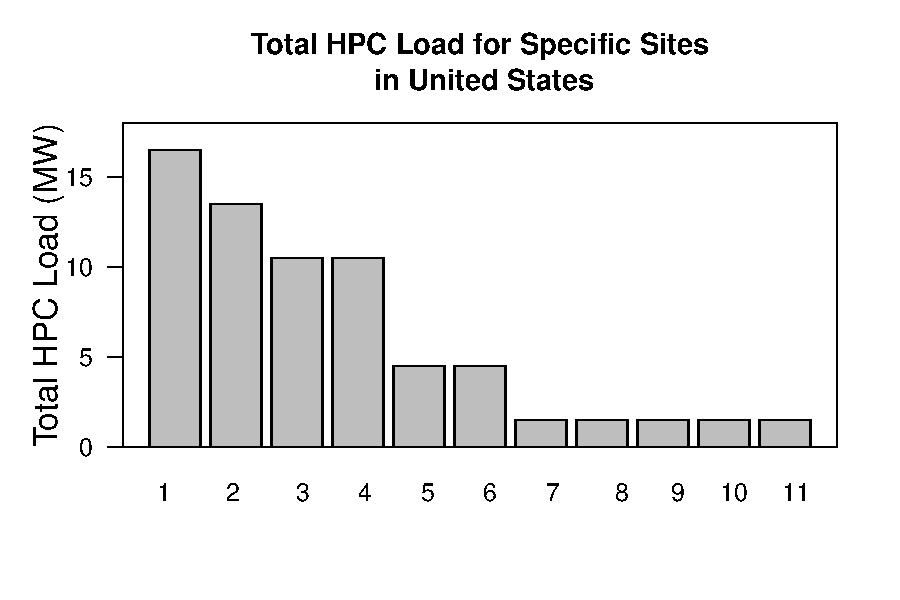
\includegraphics[scale=0.62]{figs/loadgraphUS.pdf}}
\caption{Total Load at at SCs in United States}
\label{fig:USload}
\vspace{0.9cm}
\frame{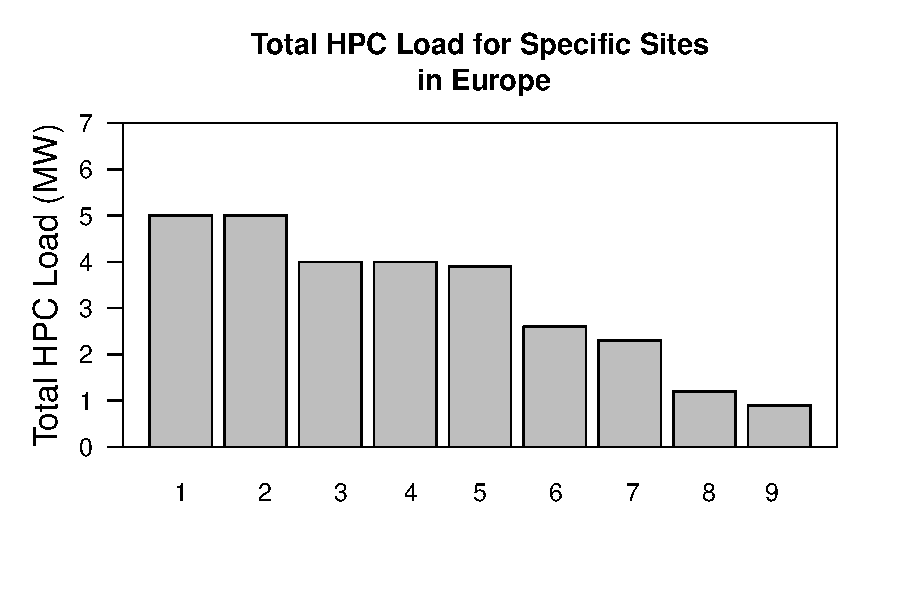
\includegraphics[scale=0.62]{figs/loadgraphEU.pdf}}
\caption{Total Load at at SCs in Europe}
\label{fig:EUload}
\end{center}
\end{figure}

We noted that none of the European SCs communicated about grid integration potential (e.g., demand response) and available flexibility with their associated ESPs. Additionally, there was little interest in a tighter integration with the ESPs.

\begin{figure}[ht!]
\begin{center}
\frame{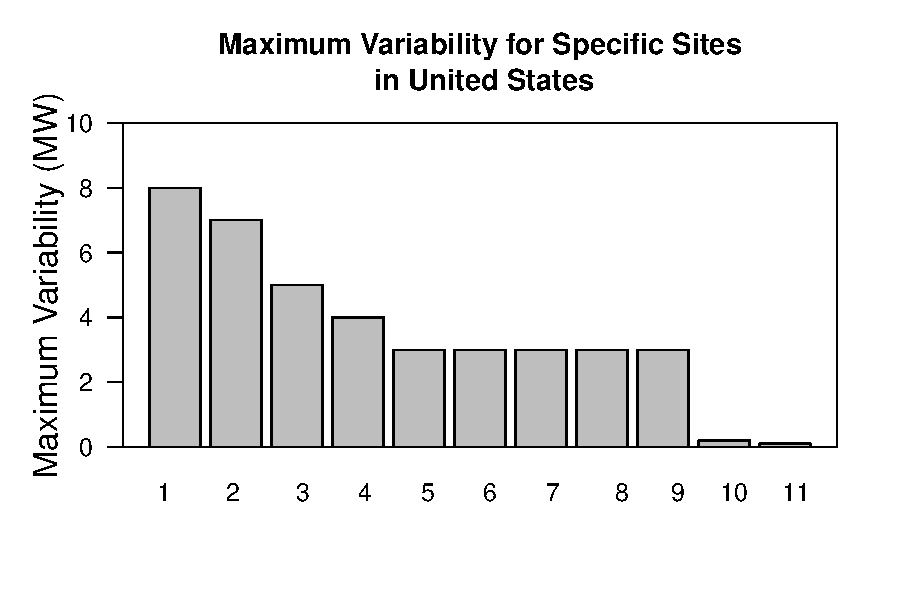
\includegraphics[scale=0.62]{figs/vargraphUS.pdf}}
\caption{Maximum Variability at at SCs in United States}
\label{fig:USvar}
\vspace{0.9cm}
\frame{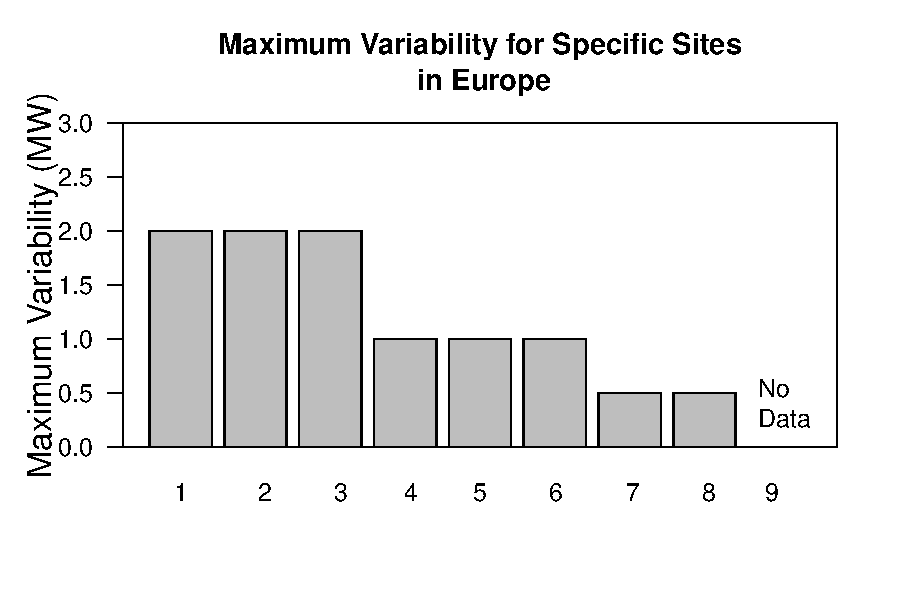
\includegraphics[scale=0.62]{figs/vargraphEU.pdf}}
\caption{Maximum Variability at at SCs in Europe}
\label{fig:EUvar}
\end{center}
\end{figure}

Figures \ref{fig:USload} and \ref{fig:EUload} depict the total load in megawatts for each of the respondents in the United States and in Europe. Most supercomputing sites have a total load of under 5 MW (sixteen out of twenty). Four of the surveyed supercomputing sites had a total load of over 10 MW. \\

Both United States and Europe had power swings and fluctuations of a few megawatts. In our questionnaire, we asked respondents to report the maximum variability that they have experienced in their SCs. The results of these for United States as well as Europe are shown in Figures \ref{fig:USvar} and \ref{fig:EUvar} respectively. In the United States, three of the eleven sites surveyed had maximum variability of over 5 MW. For our United States respondents, the minimal option for reporting this was ``Less than 3 MW'', because of which we could not capture less intense power swings. In the European survey, we allowed the respondents to provide a more accurate value, and as shown in Figure \ref{fig:EUvar}, we observed power swings in the range of half a megawatt to about 2 MW. Almost all of the respondents reported that this variability is due to maintenance cycles, and that it can be scheduled \emph{day-ahead} if necessary.
